Considera los dos triángulos que se muestran abajo en la Figura \ref{fig:20230323152030} (los triángulos no están dibujados a escala).

\begin{minipage}{0.6\textwidth}
    \textbf{¿Los dos triángulos son congruentes?}\\
    \emph{Escoge 1 respuesta:}\\

    \begin{choices}
        \choice Sí.
        \choice No.
        \CorrectChoice No hay suficiente información para decidir.
    \end{choices}
\end{minipage}%
\begin{minipage}{0.35\textwidth}
    \begin{figure}[H]
        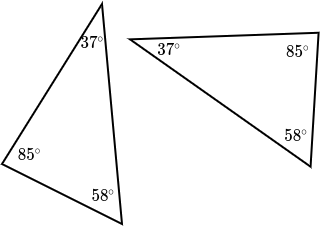
\includegraphics[width=0.8\linewidth]{../images/20230323152030}
        \caption{}
        \label{fig:20230323152030}
    \end{figure}
\end{minipage}

\begin{solutionbox}{6cm}\footnotesize
    \begin{minipage}[t][][t]{0.6\textwidth}
        Dos triángulos son congruentes si tienen la misma forma y tamaño. En otras palabras, dos triángulos son congruentes si todos los lados y ángulos correspondientes son congruentes.
        Sin embargo, no necesitamos mostrar la congruencia de todos los lados y ángulos correspondientes para demostrar que dos triángulos son congruentes. Los criterios de congruencia (LLL, LAL, ALA) y el teorema AAL son atajos útiles para determinar congruencia de triángulos. (Ver criterios al inicio de esta guía).
        En este caso, vemos que cada ángulo en el primer triángulo es congruente con un ángulo en el segundo triángulo. Nos dan AAA, que no es un criterio de congruencia.
        Si los tres ángulos de un triángulo son congruentes con los ángulos correspondientes de otro triángulo, entonces los triángulos son semejantes pero no necesariamente congruentes entre sí. En la siguiente imagen, observa que los triángulos tienen la misma forma, pero no son del mismo tamaño.
        Los triángulos podrían ser congruentes si las longitudes de los lados correspondientes en cada triángulo fueran congruentes, pero a menos que sepamos esto, no podemos sacar conclusiones.
        \textbf{No hay suficiente información para decir si los triángulos son congruentes o no.}
    \end{minipage}\hfill
    \begin{minipage}[t][][t]{0.35\textwidth}
        \begin{figure}[H]
            \centering
            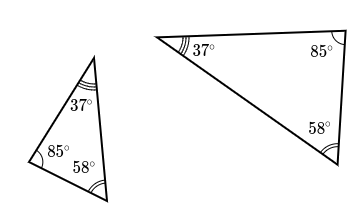
\includegraphics[width=0.8\linewidth]{../images/20230323153219}
            \caption{}
            \label{fig:20230323153219}
        \end{figure}
    \end{minipage}
\end{solutionbox}